To build a classifier to recognize different actions, we used \textit{mlpy} library. mlpy is Machine Learning library for python. This library provides a variety of ML algorithms and tools to perform ML on data.\\
The algorithm used in this project is Linear Support Vector Machine which was trained over 5 principle components of the input data.
\subsubsection*{Principle Component Analysis}
Input vector consists of 12 features for every image sequence, 7 HuMoments and 5 area measures over time. Dataset lies in 12 dimension space which is more than what really data represents therefore we performed PCA on the dataset to reduce dimensionality of the original dataset. In figure \ref{fig:pca} we can see that only first 5 Principle Components contribute to most variation in the dataset. Using these components we project the dataset into lower 5 dimension manifold.\\

\begin{figure}[htp]
\begin{center}
\leavevmode
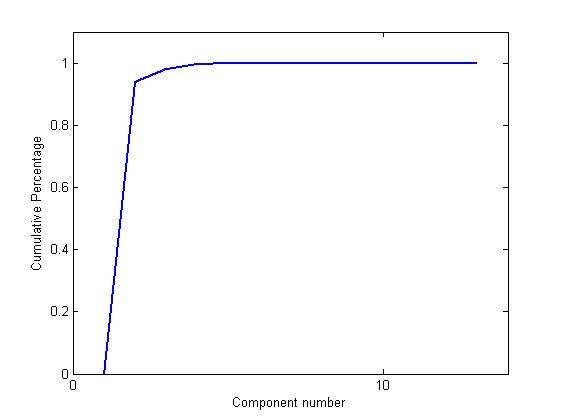
\includegraphics[width=0.6\textwidth] {pca.jpg}
\end{center}
\caption{Cumulative Percentage PCs}
\label{fig:pca}
\end{figure}

\textit{mlpy} library provides a simple API to perform PCA.
\subsubsection*{SVM}
projected data is used to train a linear SVM. The algorithm is an implementation of \textit{multi-class support vector classification by Crammer and Singer}. This algorithm is also available in mlpy library.\\
We also tested Logistic Regression however SVM outperformed. The results for both classifiers are presented in results section.
\subsubsection*{Cross Validation}
In order to report correct performance measures for our classifier we utilized Leave-one-out Cross-Validation. The algorithm at each step leaves one instance of data out and performs training on the remaining data. Using the trained classifier test instance is checked and results accumulated for all dataset.

Summary of the algorithms and parameters used in classification module is presented in table \ref{tbl:classification}.
\begin{table}
\begin{tabular}{|c|c|}
\hline 
Preprocessing: & Principal Component Analysis with 5 Components \\ 
\hline 
Training Algorithm & Multi-class SVM \\ 
\hline 
Performance Measure & Leave-One-Out Cross-Validation \\ 
\hline 

\end{tabular} 
\caption{Summary of Classification Module parameters and algorithms}
\label{tbl:classification}
\end{table}